\section{Problem 2}
\subsection{Technics}

    \begin{frame}
        \frametitle{Using Eigen Library for C++}

        \begin{itemize}
            \item Compute eigenvalues using SelfAjointEigenSolver.
            \item Check if \(VV^\dagger = V^\dagger V = I\). If not, do Gram-Schmidt orthogonalization.
        \end{itemize}

    \end{frame}

    \begin{frame}
    \frametitle{Program Results}
    
    \begin{figure}
        \centering
        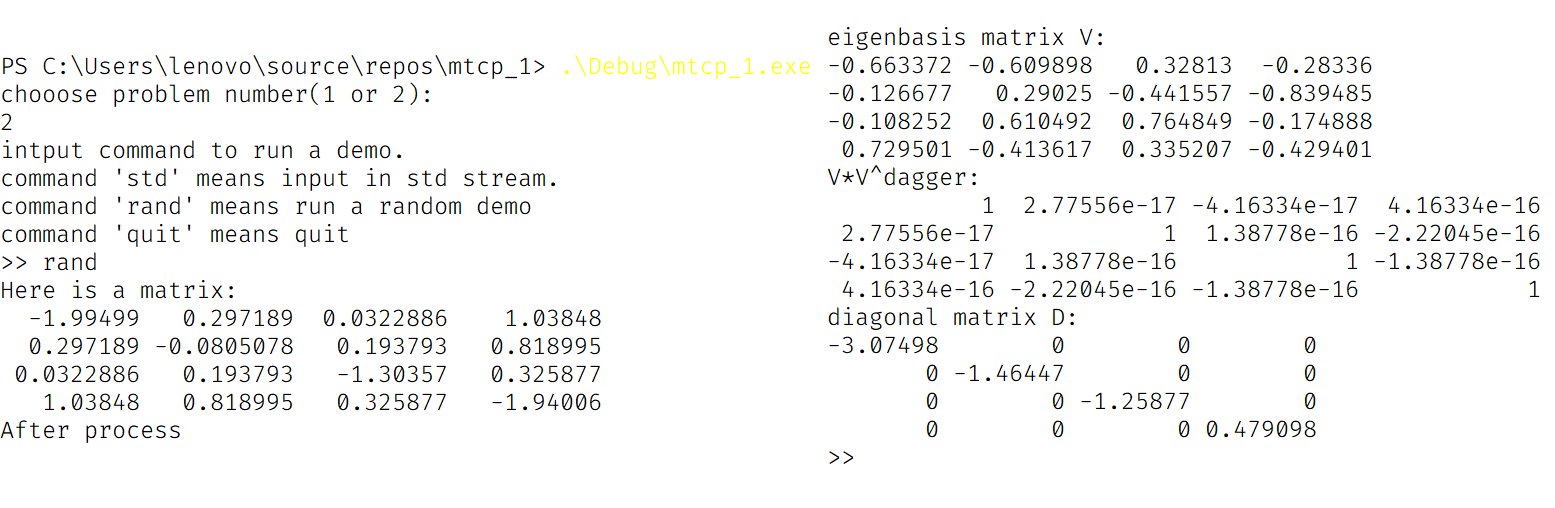
\includegraphics[height = 0.8\textheight]{img/result2.png}
    \end{figure}
\end{frame}

\begin{frame}[fragile]          % 注意添加 fragile 标记
    \frametitle{代码块}
    % 代码块参数:语言,标题
    % 请减少代码初始的缩进
    \begin{codeblock}{c++}{C++代码}
#include<iostream>

int main(){
// Console Output
std::cout << "Hello, SJTU!" << std::endl;
return 0;
}
    \end{codeblock}
\end{frame}

